\section{USB-to-UART}
\label{sec:usbtouart}

\fig{ubstouart}{USB-to-UART-Adapter}{\gls{USB-to-UART}-Adapter}{\textwidth}{Schuh/Pictures/usbtouart-hard}

\subsection{Allgemeines}
\label{sec:usbtouart-allgemeines}
Der Adapter ermöglicht den Datenaustausch via USB zwischen einem PC und seriellen Geräten (z.B.: Mikrocontroller mit UART). Darüber hinaus soll dieses Modul eine einfache Programmierung und Kommunikation mit einem NEXTION-Display ermöglichen. Die Kommunikation zwischen den beiden Endgeräten wird durch den FTDI-Chip FT232RL ermöglicht. Dieser Chip ermöglicht eine Emulation einer seriellen Schnittstelle über USB.

\subsection{Schnittstellen}
\label{sec:usbtouart-schnittstellen}

Der \gls{USB-to-UART}-Adapter verfügt über die in \fref{tab:usbtouart-schnittstellen} angegebenen Schnittstellen, welche wie in \fref{fig:usbtouart-plan} zu sehen platziert sind.

\tab{usbtouart-schnittstellen}{Schnittstellen des USB-to-UART-Adapter}{Schnittstellen des \gls{USB-to-UART}-Adapter}{|c|p{10cm}|}{
    \hline
    \textbf{Schnittstelle} & \textbf{Funktion}\\
    \hline
    UART & Senden und Empfangen von Daten vom Terminal oder Controller\\
    \hline
    USB-B & Weiterleitung der Daten zum PC\\
    \hline
}

\fig{usbtouart-plan}{Übersichtsplan des USB-to-UART-Adapter}{Übersichtsplan des \gls{USB-to-UART}-Adapter}{0.75\textwidth}{Schuh/Pictures/usbtouart}

\subsubsection{UART}
Die UART-Schnittstelle wurde hardwaremäßig zweimal herausgeführt. Einmal zu der Stiftleiste X2 (\fref{fig:usbtouart-uart1}) und einmal zum Header X3 (\fref{fig:usbtouart-uart2}). Die Stiftleiste X2 (\fref{fig:usbtouart-uart1}) dient zur Kommunikation mit den diversen UART-Interfaces auf der \gls{Basisplatine}, als auch zu Kommunikation mit der UART-Schnittstelle auf dem \gls{Core-Modul}. Der Header X3 (\fref{fig:usbtouart-uart2}) dient zur Programmierung und Kommunikation mit einem NEXTION-Display.

\begin{figure}[H]
    \centering
    \subfloat[Schematic\label{fig:usbtouart-uart1}]{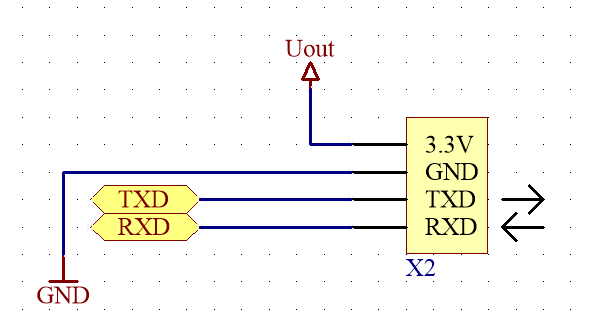
\includegraphics[width=.4\linewidth]{Schuh/Pictures/usbtouart-uart1}}\qquad
    \subfloat[Schematic für NEXTION-Display\label{fig:usbtouart-uart2}]{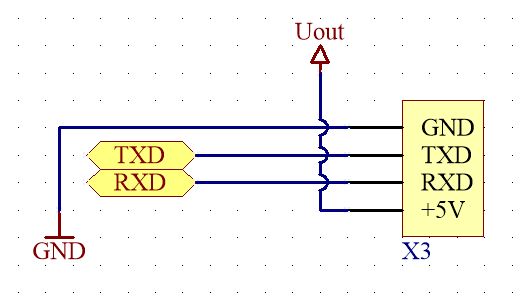
\includegraphics[width=.4\linewidth]{Schuh/Pictures/usbtouart-uart2}}\qquad
    \subfloat[Hardware\label{fig:usbtouart-uart-hard}]{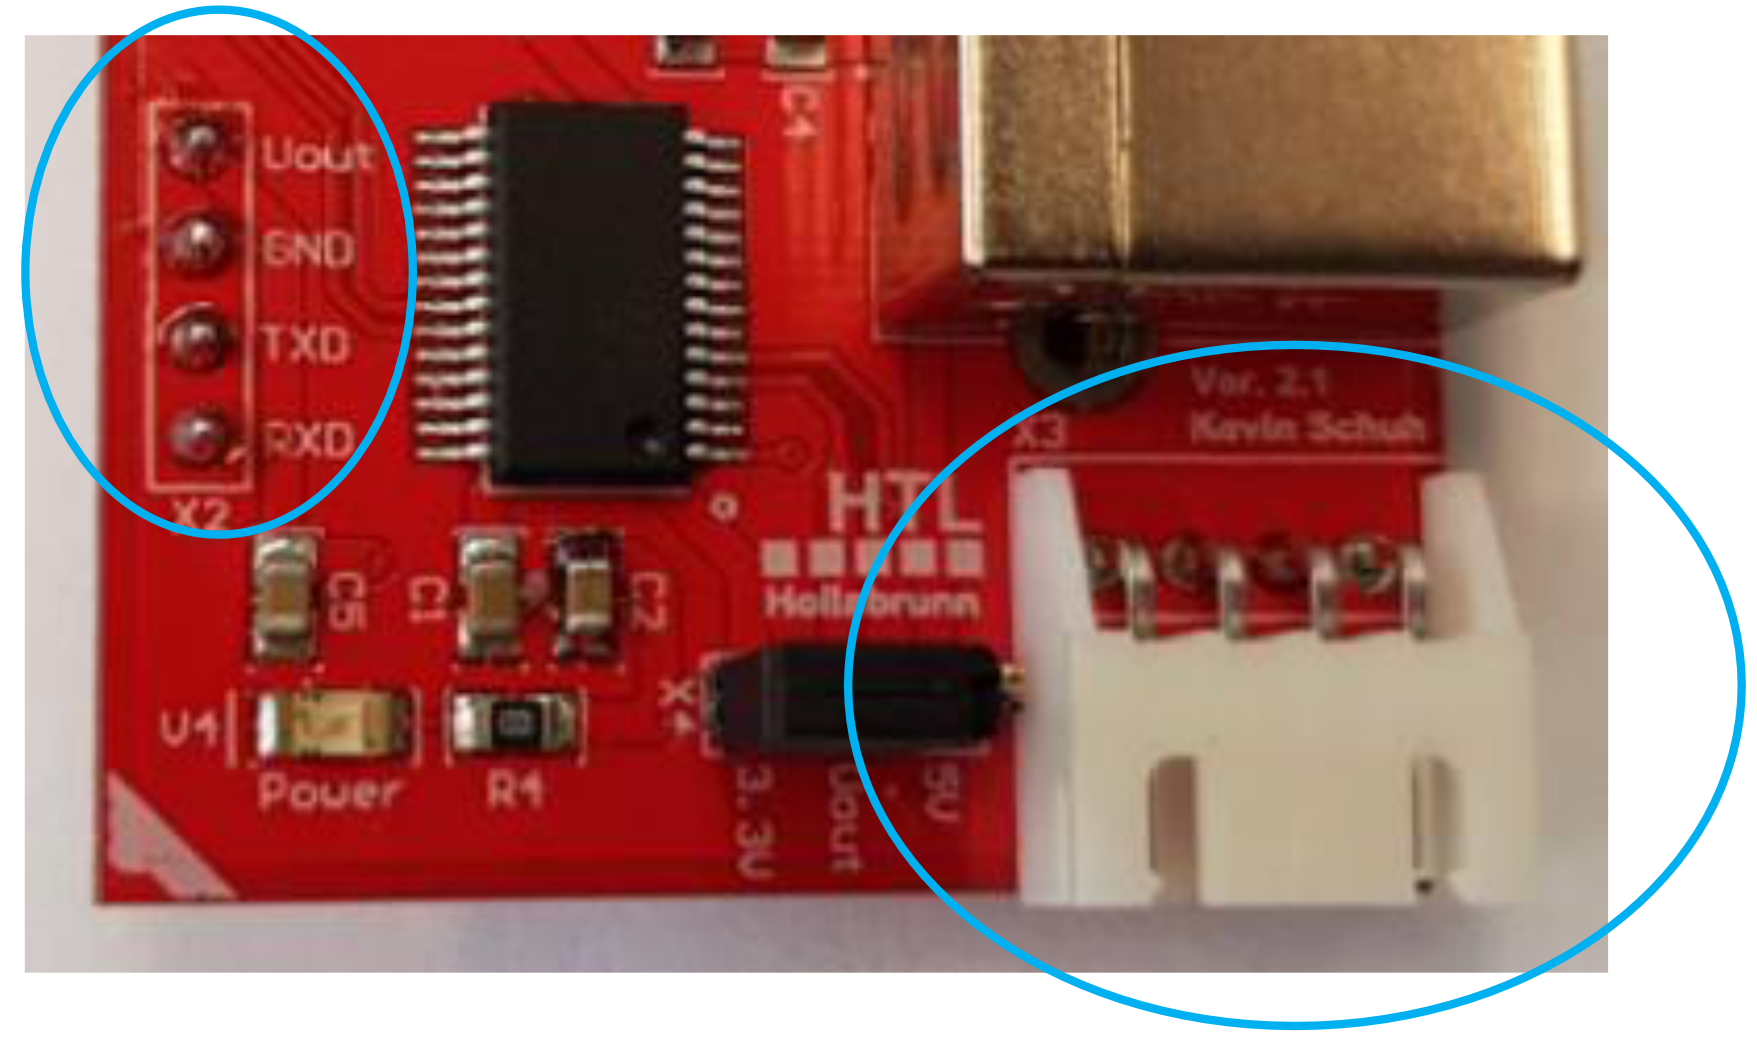
\includegraphics[width=.3\linewidth]{Schuh/Pictures/usbtouart-uart-hard}}\qquad
    \caption[UART des USB-to-UART-Adapter]{UART des \gls{USB-to-UART}-Adapter}
    \label{fig:usbtouart-uart}
\end{figure}

\subsubsection{Spannungsversorgung}
Die Betriebsspannungsversorgung von \unit{+5}{\volt} sollte prinzipiell nur über die USB-B Buchse X1 (\fref{fig:usbtouart-spannung1}) zur Verfügung gestellt werden. Diese Spannungsversorgung wird auch zur Programmierung und Kommunikation mit dem NEXTION-Display oder mit anderen \unit{5}{\volt} Interfaces benötigt. Zur Überprüfung ob das Modul mit Spannung versorgt wird, wurde die LED V4 (\fref{fig:usbtouart-spannung2}) zur optischen Kontrolle eingebaut. Wenn das Modul mit Spannung über die USB-B Buchse versorgt wird, beginnt diese zu leuchten.

Es gibt zusätzlich zur Betriebsspannung noch eine vom FTDI-Chip generierte \unit{+3,3}{\volt} Spannungsversorgung, welche zur Kommunikation mit den verwendeten UART-Interfaces auf der \gls{Basisplatine} und dem \gls{Core-Modul} benötigt wird. Der Hardwareaufbau erlaubt es je nach verwendeten Interface, durch Setzen von einem Jumper auf der Stiftleiste X4 (\fref{fig:usbtouart-spannung3}) die Betriebsspannungen für das entsprechende Interface selbst zu wählen. Durch Verbinden des Pin1 mit dem Pin2, wird am Ausgang eine Spannung von \unit{+5}{\volt} ausgegeben. Durch Verbinden des Pin2 mit dem Pin3, wird am Ausgang eine Spannung von \unit{+3,3}{\volt} ausgegeben.

\begin{figure}[H]
    \centering
    \subfloat[Schematic\label{fig:usbtouart-spannung1-schem}]{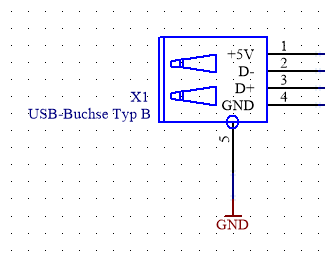
\includegraphics[width=.5\linewidth]{Schuh/Pictures/usbtouart-spannung1}}\qquad
    \subfloat[Hardware\label{fig:usbtouart-spannung1-hard}]{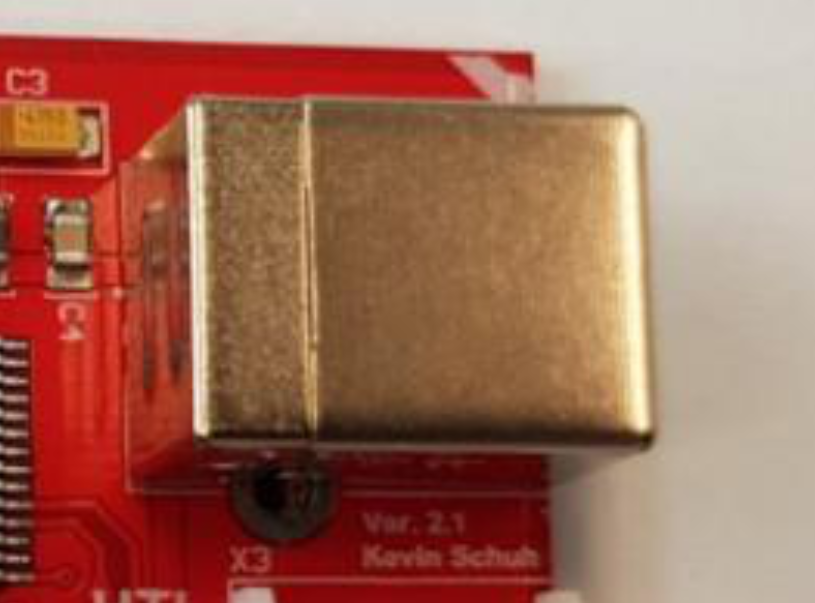
\includegraphics[width=.3\linewidth]{Schuh/Pictures/usbtouart-spannung1-hard}}\qquad
    \caption[Spannungsversorgung des USB-to-UART-Adapter]{Spannungsversorgung des \gls{USB-to-UART}-Adapter}
    \label{fig:usbtouart-spannung1}
\end{figure}

\begin{figure}[H]
    \centering
    \subfloat[Schematic\label{fig:usbtouart-spannung2-schem}]{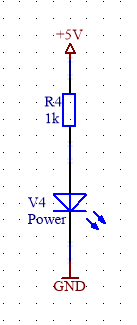
\includegraphics[width=.25\linewidth]{Schuh/Pictures/usbtouart-spannung2}}\qquad
    \subfloat[Hardware\label{fig:usbtouart-spannung2-hard}]{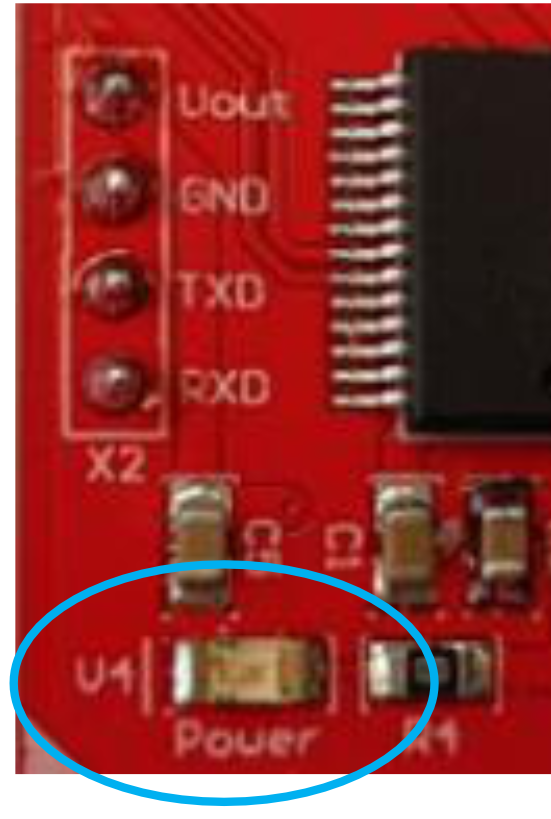
\includegraphics[width=.3\linewidth]{Schuh/Pictures/usbtouart-spannung2-hard}}\qquad
    \caption[Spannungsversorgungs-LED des USB-to-UART-Adapter]{Spannungsversorgungs-LED des \gls{USB-to-UART}-Adapter}
    \label{fig:usbtouart-spannung2}
\end{figure}

\begin{figure}[H]
    \centering
    \subfloat[Schematic\label{fig:usbtouart-spannung3-schem}]{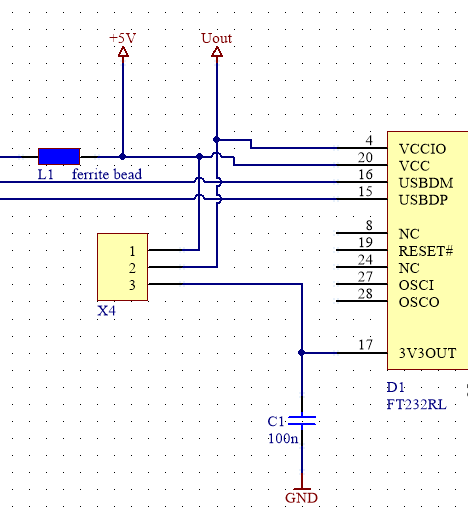
\includegraphics[width=.5\linewidth]{Schuh/Pictures/usbtouart-spannung3}}\qquad
    \subfloat[Hardware\label{fig:usbtouart-spannung3-hard}]{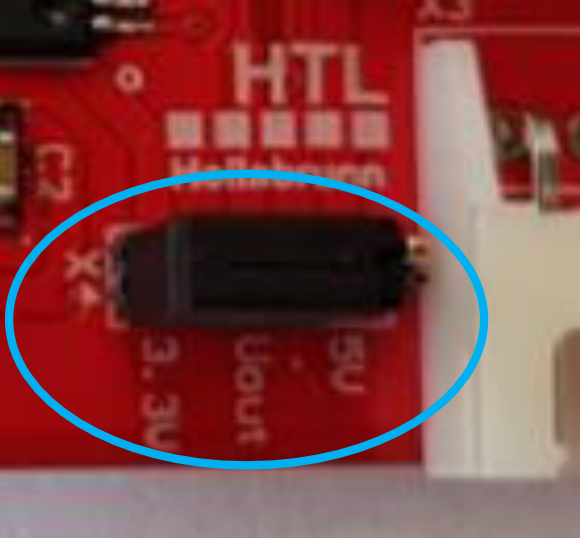
\includegraphics[width=.3\linewidth]{Schuh/Pictures/usbtouart-spannung3-hard}}\qquad
    \caption[Spannungsversorgungs-Jumper des USB-to-UART-Adapter]{Spannungsversorgungs-Jumper des \gls{USB-to-UART}-Adapter}
    \label{fig:usbtouart-spannung3}
\end{figure}

\subsubsection{Status-LEDs}
Die Status-LEDs V1 und V2 (\fref{fig:usbtouart-leds}) dienen zu optischen Kontrolle, ob Daten zwischen den Sender den Empfänger ausgetauscht werden. Die LED V1 leuchtet, sobald Daten über das Modul gesendet werden. Die LED V2 hingegen zeigt an ob Daten zum Modul gelangen.

\begin{figure}[H]
    \centering
    \subfloat[Schematic\label{fig:usbtouart-leds-schem}]{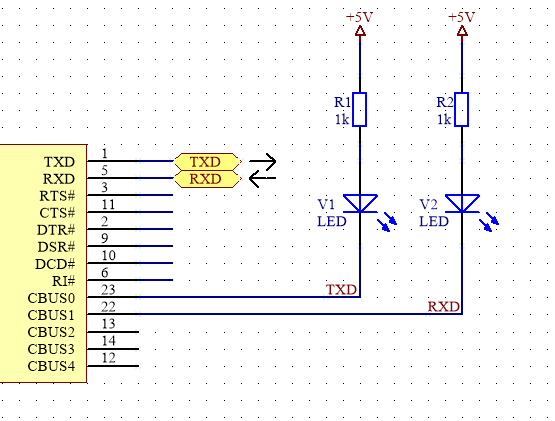
\includegraphics[width=.5\linewidth]{Schuh/Pictures/usbtouart-leds}}\qquad
    \subfloat[Hardware\label{fig:usbtouart-leds-hard}]{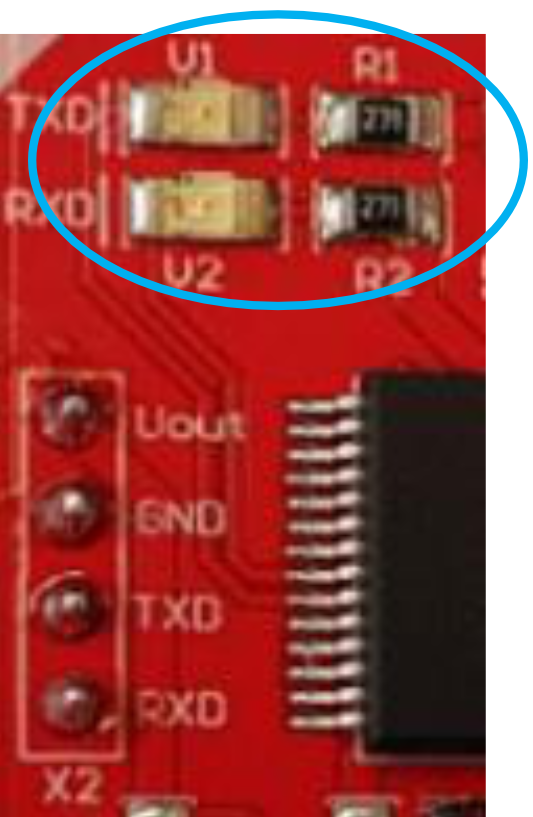
\includegraphics[width=.3\linewidth]{Schuh/Pictures/usbtouart-leds-hard}}\qquad
    \caption[Status-LEDs des USB-to-UART-Adapter]{Status-LEDs des \gls{USB-to-UART}-Adapter}
    \label{fig:usbtouart-leds}
\end{figure}

\subsubsection{FTDI-Chip}
Durch den FTDI-Chip FT232RL wird die eine Verwendung einer seriellen Schnittstelle über USB-Geräte ermöglicht.

\begin{figure}[H]
    \centering
    \subfloat[Schematic\label{fig:usbtouart-ftdi-schem}]{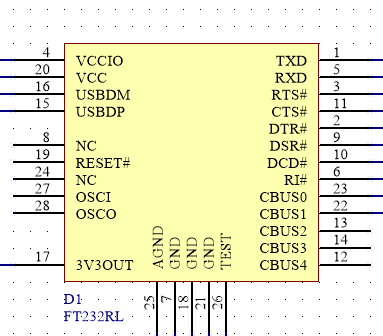
\includegraphics[width=.5\linewidth]{Schuh/Pictures/usbtouart-ftdi}}\qquad
    \subfloat[Hardware\label{fig:usbtouart-ftdi-hard}]{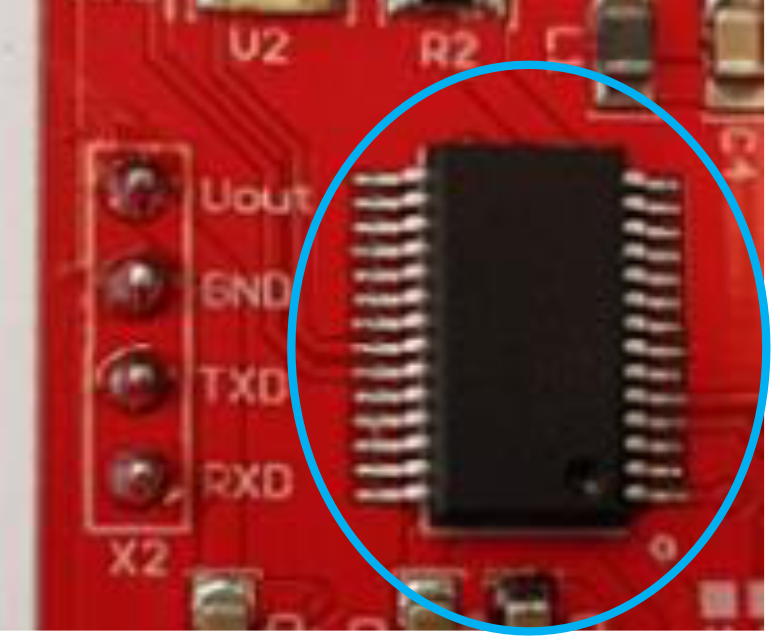
\includegraphics[width=.3\linewidth]{Schuh/Pictures/usbtouart-ftdi-hard}}\qquad
    \caption[FTDI-Chip des USB-to-UART-Adapter]{FTDI-Chip des \gls{USB-to-UART}-Adapter}
    \label{fig:usbtouart-ftdi}
\end{figure}

\subsubsubsection{Blockschaltbild}
Wie anhand des Blockschaltbildes ersichtlich ist, ist bereits ein \unit{3,3}{\volt} LDO-Regulator im FTDI-Chip eingebaut. Daher kann dieser die Ausgangsspannung von \unit{+3,3}{\volt} selbstständig generieren.

\fig{usbtouart-ftdi-bsb}{Blockschaltbild des FTDI-Chips}{Blockschaltbild des FTDI-Chips \cite{ftdi:ft232r}}{\textwidth}{Schuh/Pictures/usbtouart-ftdi-bsb}

\subsubsection{Pinbelegung}
\begin{table}[H]
    \centering
    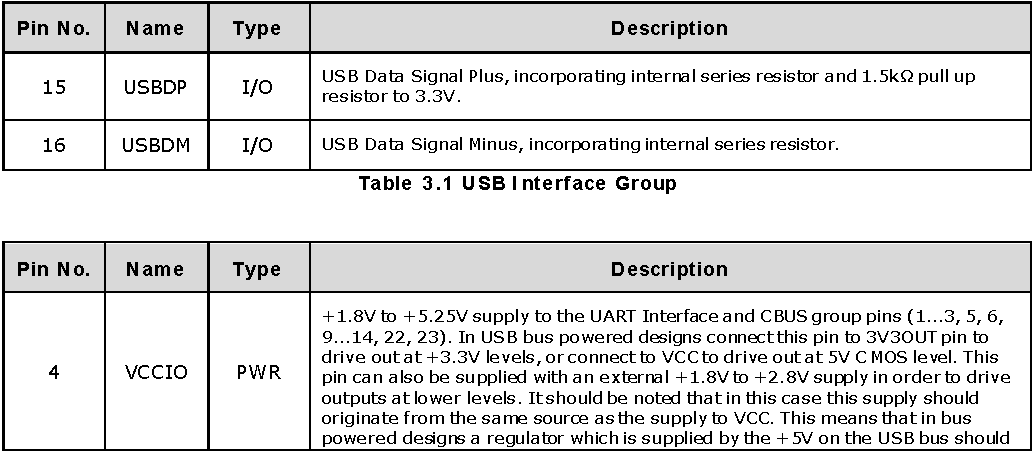
\includegraphics[width=\textwidth]{Schuh/Pictures/usbtouart-ftdi-pin1}
    \caption[Pinbelegung des FTDI]{Pinbelegung des FTDI \cite{ftdi:ft232r}}
    \label{tab:usbtouart-ftdi-pin}
\end{table}
\begin{table}[H]\ContinuedFloat
    \centering
    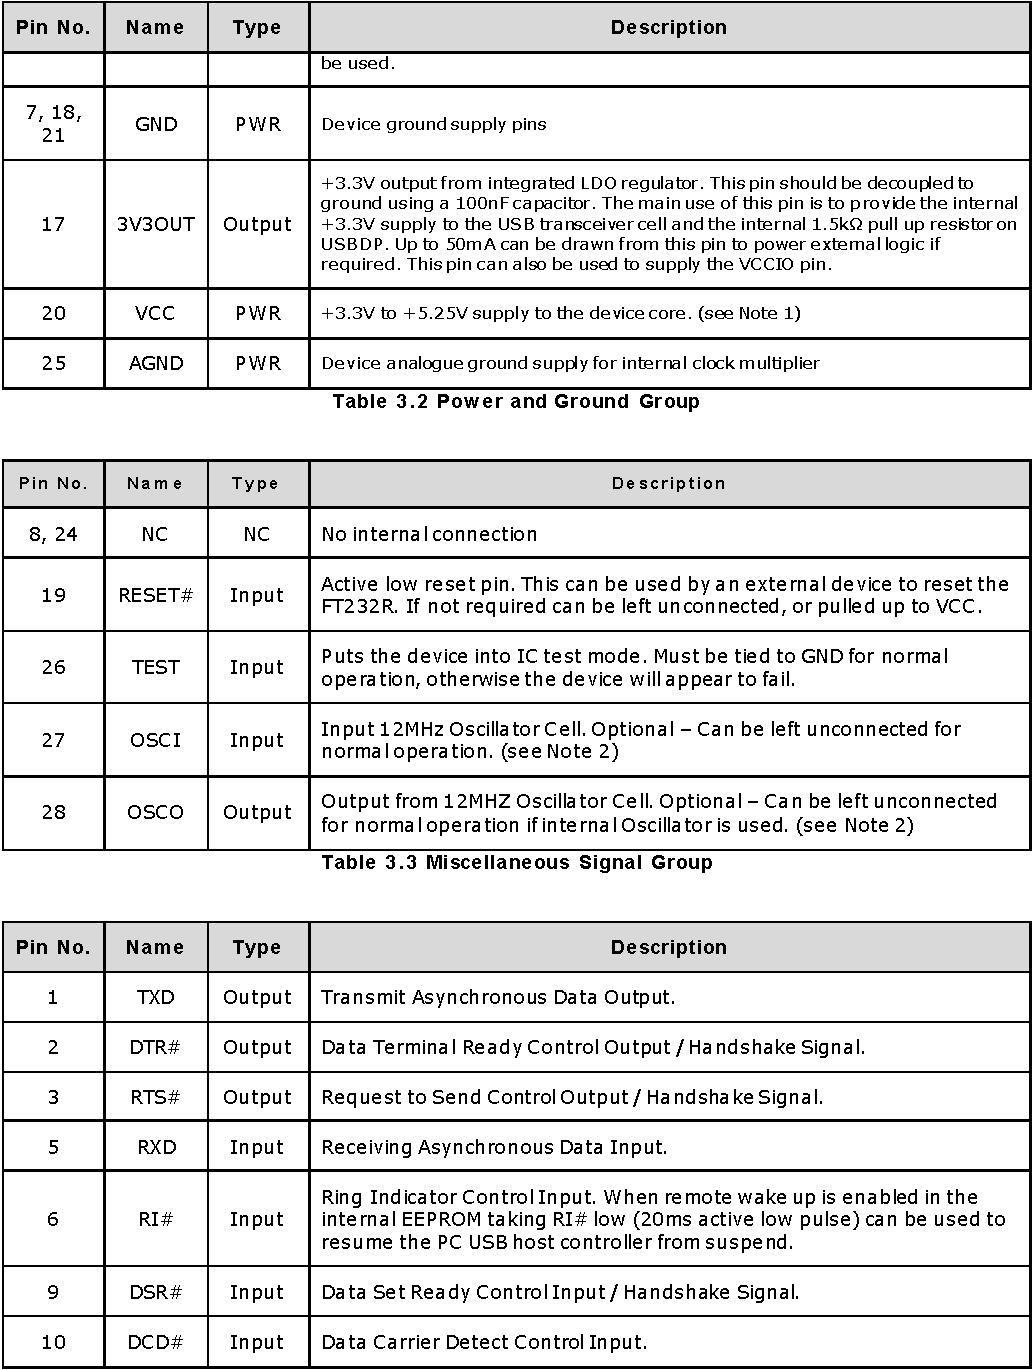
\includegraphics[width=\textwidth]{Schuh/Pictures/usbtouart-ftdi-pin2}
    \caption[Pinbelegung des FTDI]{Pinbelegung des FTDI \cite{ftdi:ft232r}}
\end{table}
\begin{table}[H]\ContinuedFloat
    \centering
    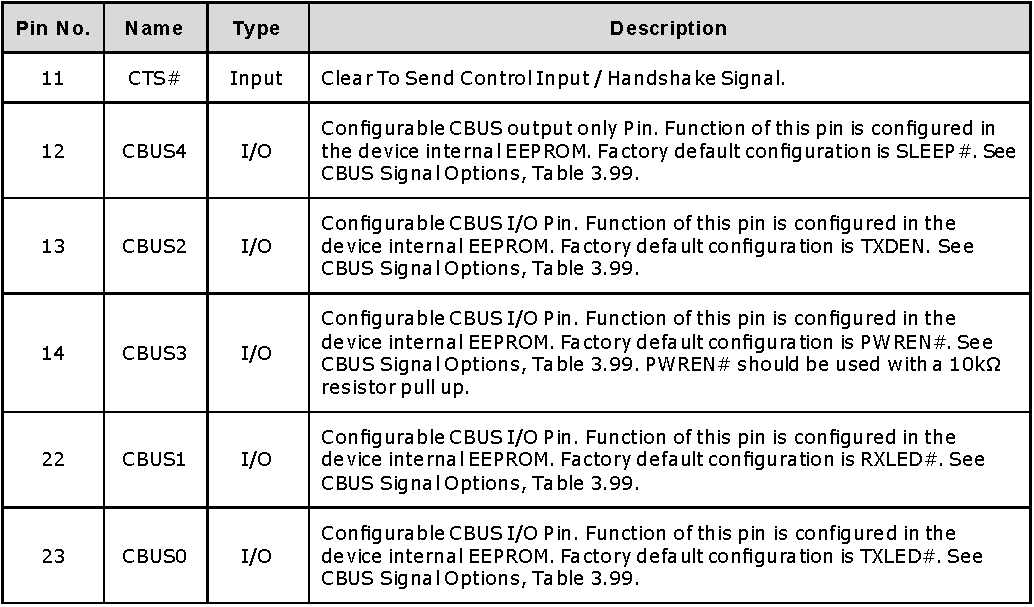
\includegraphics[width=\textwidth]{Schuh/Pictures/usbtouart-ftdi-pin3}
    \caption[Pinbelegung des FTDI]{Pinbelegung des FTDI \cite{ftdi:ft232r}}
\end{table}

\subsection{Gesamtschaltung}
\label{sec:usbtouart-schaltung}
\fig{usbtouart-schaltung}{Gesamtschaltung des USB-to-UART-Adapter}{Gesamtschaltung des \gls{USB-to-UART}-Adapter}{0.7\textwidth}{Schuh/Pictures/usbtouart-schaltung}

\subsection{Leiterplattenlayout}
\label{sec:usbtouart-leiterplattenlayout}
\subsubsection{Bauteilseite}
\fig{usbtouart-lbauteilseite}{Layout Bauteilseite des USB-to-UART-Adapters}{Layout Bauteilseite des \gls{USB-to-UART}-Adapters}{0.7\textwidth}{Schuh/Pictures/usbtouart-lbauteilseite}

\subsubsection{Lötseite}
\fig{usbtouart-llötseite}{Layout Lötseite des USB-to-UART-Adapters}{Layout Lötseite des \gls{USB-to-UART}-Adapters}{0.7\textwidth}{Schuh/Pictures/usbtouart-llotseite}

\subsection{Bestückungspläne}
\label{sec:usbtouart-bestückungspläne}
\subsubsection{Bauteilseite}
\fig{usbtouart-bbauteilseite}{Bestückungsplan Bauteilseite des USB-to-UART-Adapters}{Bestückungsplan Bauteilseite des \gls{USB-to-UART}-Adapters}{0.75\textwidth}{Schuh/Pictures/usbtouart-bbauteilseite}